\documentclass[12pt]{article}
\usepackage[utf8]{inputenc}

\usepackage{algorithm}% http://ctan.org/pkg/algorithms
\usepackage{algpseudocode}% http://ctan.org/pkg/algorithmicx
\usepackage{graphicx}
\usepackage{fancyhdr}
\usepackage{setspace}
\usepackage{minted}
\usepackage{biblatex}
\usepackage{svg}
%inline verbatim%
\usepackage{fancyvrb}

\addbibresource{references.bib}

\pagestyle{fancy}

% remove header
\renewcommand{\headrulewidth}{0pt}
\fancyhead{}

% set margin
\usepackage[
  top=1in,
  bottom=1in,
  left=1.5in,
  right=1in
]{geometry} 

\begin{document}
\begin{titlepage}
   \begin{center}
        Kalamazoo College\\
        Senior Individualized Project in Computer Science
       \vspace*{3cm}
 
       \textbf{SQL query generation from decorator declared GraphQL schema}
 
       \vspace{0.5cm}
        Subtitle
 
       \vspace{1.5cm}
 
       \textbf{Joshua Gibson}
 
       \vspace{4cm}
 
       Faculty Supervisor:\\
       Dr. Eric Barth\\
       Assistant Provost and Professor of Mathematics\\
       Kalamazoo College\\
       Kalamazoo, MI
       
       \vspace{3cm}
       
       A paper submitted in partial fulfillment of the requirements for the degree of Bachelor of Arts at Kalamazoo College
       
       \vspace{2cm}
       2019
 
   \end{center}
\end{titlepage}

\pagenumbering{gobble}

%empty page
\null \newpage

\pagenumbering{roman}
\setcounter{page}{2}

\tableofcontents
\newpage

\doublespacing

\addcontentsline{toc}{section}{Acknowledgements}
\section*{Acknowledgements}
This project would not have been possible without the help of dozens of people, both during the process of the SIP and before it was even a thought.  While this is by no means an exhaustive list, there are a number of people who must be thanked by name for their help.  I of course have to start by thanking my advisor Dr. Eric Barth for taking me on as an advisee.  This project has morphed a lot since he agreed to advise me on it, but he has been fully supportive in letting the project evolve naturally.  His guidance and support through these changes has been crucial.  In helping plan my initial project for my SIP, I must also thank Professor Andrew Koehler for his similar willingness to advise a project somewhat outside of his comfort zone.

As I developed the technologies discussed in my SIP over the summer, I would not have been able to do so without the mentorship and guidance of my co-workers at Maestro.  A huge thanks goes out to John Pinkster, Ben Meden, and Tyler VanderMaas for teaching me so much about back-end development.  Additionally, I have to thank Baxter Banghart for not entertaining phone calls throughout the summer where I would excitedly plan and develop these crazy ideas about GraphQL, but also for helping push me to be a better over the last eight years we've collaborated together.

This paper itself would also not be possible without the help of many people.  Thanks to Dr. Alyce Brady for entertaining my questions throughout the SIP Seminar and offering her years of wisdom she's gained through advising CS SIPs.  Thanks to all of my fellow CS students who proofread my paper as it was in the process of being written.  Additionally, thanks to my sister Amanda Gibson, for proofreading the paper as it neared its final draft.

Finally, I have to thank those who helped me get to where I am today.  A huge thanks goes out to Dr. Kelly Schultz.  She was the teacher who inspired my passion for Computer Science at such a young age and lead me to the computer science department at Kalamazoo College.  It makes me happy to know she's still teaching and inspiring young students today.  My other CS educators at Kalamazoo College, Dr. Alyce Brady, Dr. Pam Cutter, and Dr. Gerry Howser, have also played a huge part in developing me a computer scientist.  Without their education, I would not have the skills or ambition to tackle this kind of project.   And of course, I must also thank my parents, Scott and Kristine Gibson.  They have been nothing but supportive throughout all my education, whether it was helping me dual enroll in classes to help fuel my passion for computer science, encouraging me to study music in many different contexts and venues, or supporting me throughout college. No aspect of this project would be possible without them.
\newpage

\pagenumbering{arabic}
\section{Introduction}

Programming is often a balance of writing original functionality while abstracting away often repeated code.  Instead of copying and pasting complicated code everywhere it is needed, developers seek to extract that code into its own function and reuse it through a project. This balance is a delicate game.  If the developer is left with less abstraction, they may have more control over their implementation. This lack of abstraction makes implementing new features difficult since every bit of functionality has to be re-written for each new context.  On the other hand, too much abstraction leaves the developer with little ability to adapt to their specific situation.

For small agencies that are contracted to create custom software, such as Maestro in Kalamazoo, MI, many common tasks are repeated:  services should have some form of authentication/authorization, keep track of users as they perform actions on a data set, and offer some way to request data from the service, among numerous other tasks.  While organizations over time build expertise in managing these aspects of systems, regardless of the skill of the developer, continually recreating each one of these subsystems takes a significant amount of time.  The question then becomes, what parts of this functionality could be reused across projects and what custom features should stay in individual applications.

This debate ultimately leads to what developers refer to as opinionated vs unopinionated frameworks.  An opinionated framework gives extra tools to reduce the amount of code that has to be written from scratch; however, there are often only a few correct ways to implement these features.  An unopinionated framework, on the other hand, gives the developer the basic tools needed to build their software, but the specific solutions they employ are often left up to the developer using the framework.

When I started working at Maestro as an intern and eventually Apprentice Software Engineer, the team I was a part of did have a standard way to build web servers, but they did not have framework in code to enforce those standards.  Each project was implemented in a very similar way, but features were still duplicated across each application.  For this reason, we have started to plan an opinionated framework that is specific to our team and would abstract away this repeated code.

As these framework conversations were beginning to develop, I also became interested in how to automate the translation of GraphQL queries into SQL queries.  These two languages, which are discussed below, are two common languages used to request data from a remote service.  GraphQL is focused on the communication between web browsers and web servers, whereas SQL is a language for requesting data from relational databases.  This translation functionality would allow web clients to request data from a server in any shape they desired.  Instead of the web server having to define queries for each shape of data needed by the client, the server could just respond dynamically to any data requested.  As I continued to investigate this feature, the applicability to an opinionated framework became clear.

In this paper, I will go into depth on my attempts to create a framework to automate the data fetching functionality of a web server. This framework will make it simple for a developer to define data types to be available in their web server and have those data types immediately available for clients to read, write, and update.  With this baseline functionality, duplicated code related to these operations can be removed from the software and will enable developers to maintain less code and develop more features.  This logic, however, is not specific to any project.  As will be discussed, the idea for this framework began in an independent project, was inspired by a project for Maestro, and has now developed into a project of its own.  The generality of this framework should allow it to be used for any application that needs a web server that exposes data from a database.

\section{Technologies}
Due to the varied background of those who tend to read senior individualized projects, this section seeks to introduce many of the technologies used and referenced throughout this paper.  Should the reader feel like they have a strong grasp on the following technologies, they may skip over these sections without missing content crucial to the rest of the paper.

\subsection{GraphQL}
The main technology motivating this project is GraphQL, a query language developed by Facebook in 2012 \cite{byronKeynoteBriefHistory2019}.  This language, in comparison to querying languages such as SQL (Structured Query Language), is designed to be exposed as to the web as a public set of defined functions.  Due to security concerns, SQL has been secured and users have been prevented from sending SQL queries directly to a database.  This allows GraphQL to be a public Application Program Interface (API), which is essentially a contract of what functions are available for a given piece of software.  GraphQL servers can define the available queries and mutations for the server, and the client is then only allowed to request those functions to be run by the server.

\subsubsection{Language Structure}

The unique aspect of GraphQL is that when the client requests data from the API, the client requests the shape of the response.  This means that rather than the server defining the exact data that it will provide, the client has the freedom to adapt the data requested.

Another unique part of the language is that data accessible by the API is represented as a graph of connected data types.  You could imagine each type of requestable data being a node on a graph where the edges represent relationships between the data.  When combining the ability to dynamically request data from the server and being able to request related data, the power of GraphQL becomes evident.  Since the client requests exactly what it wants and can receive all the related data in one request, the number of requests to the server is dramatically reduced and no extraneous data is sent to the client.

\begin{figure}[htbp]
    \centering
    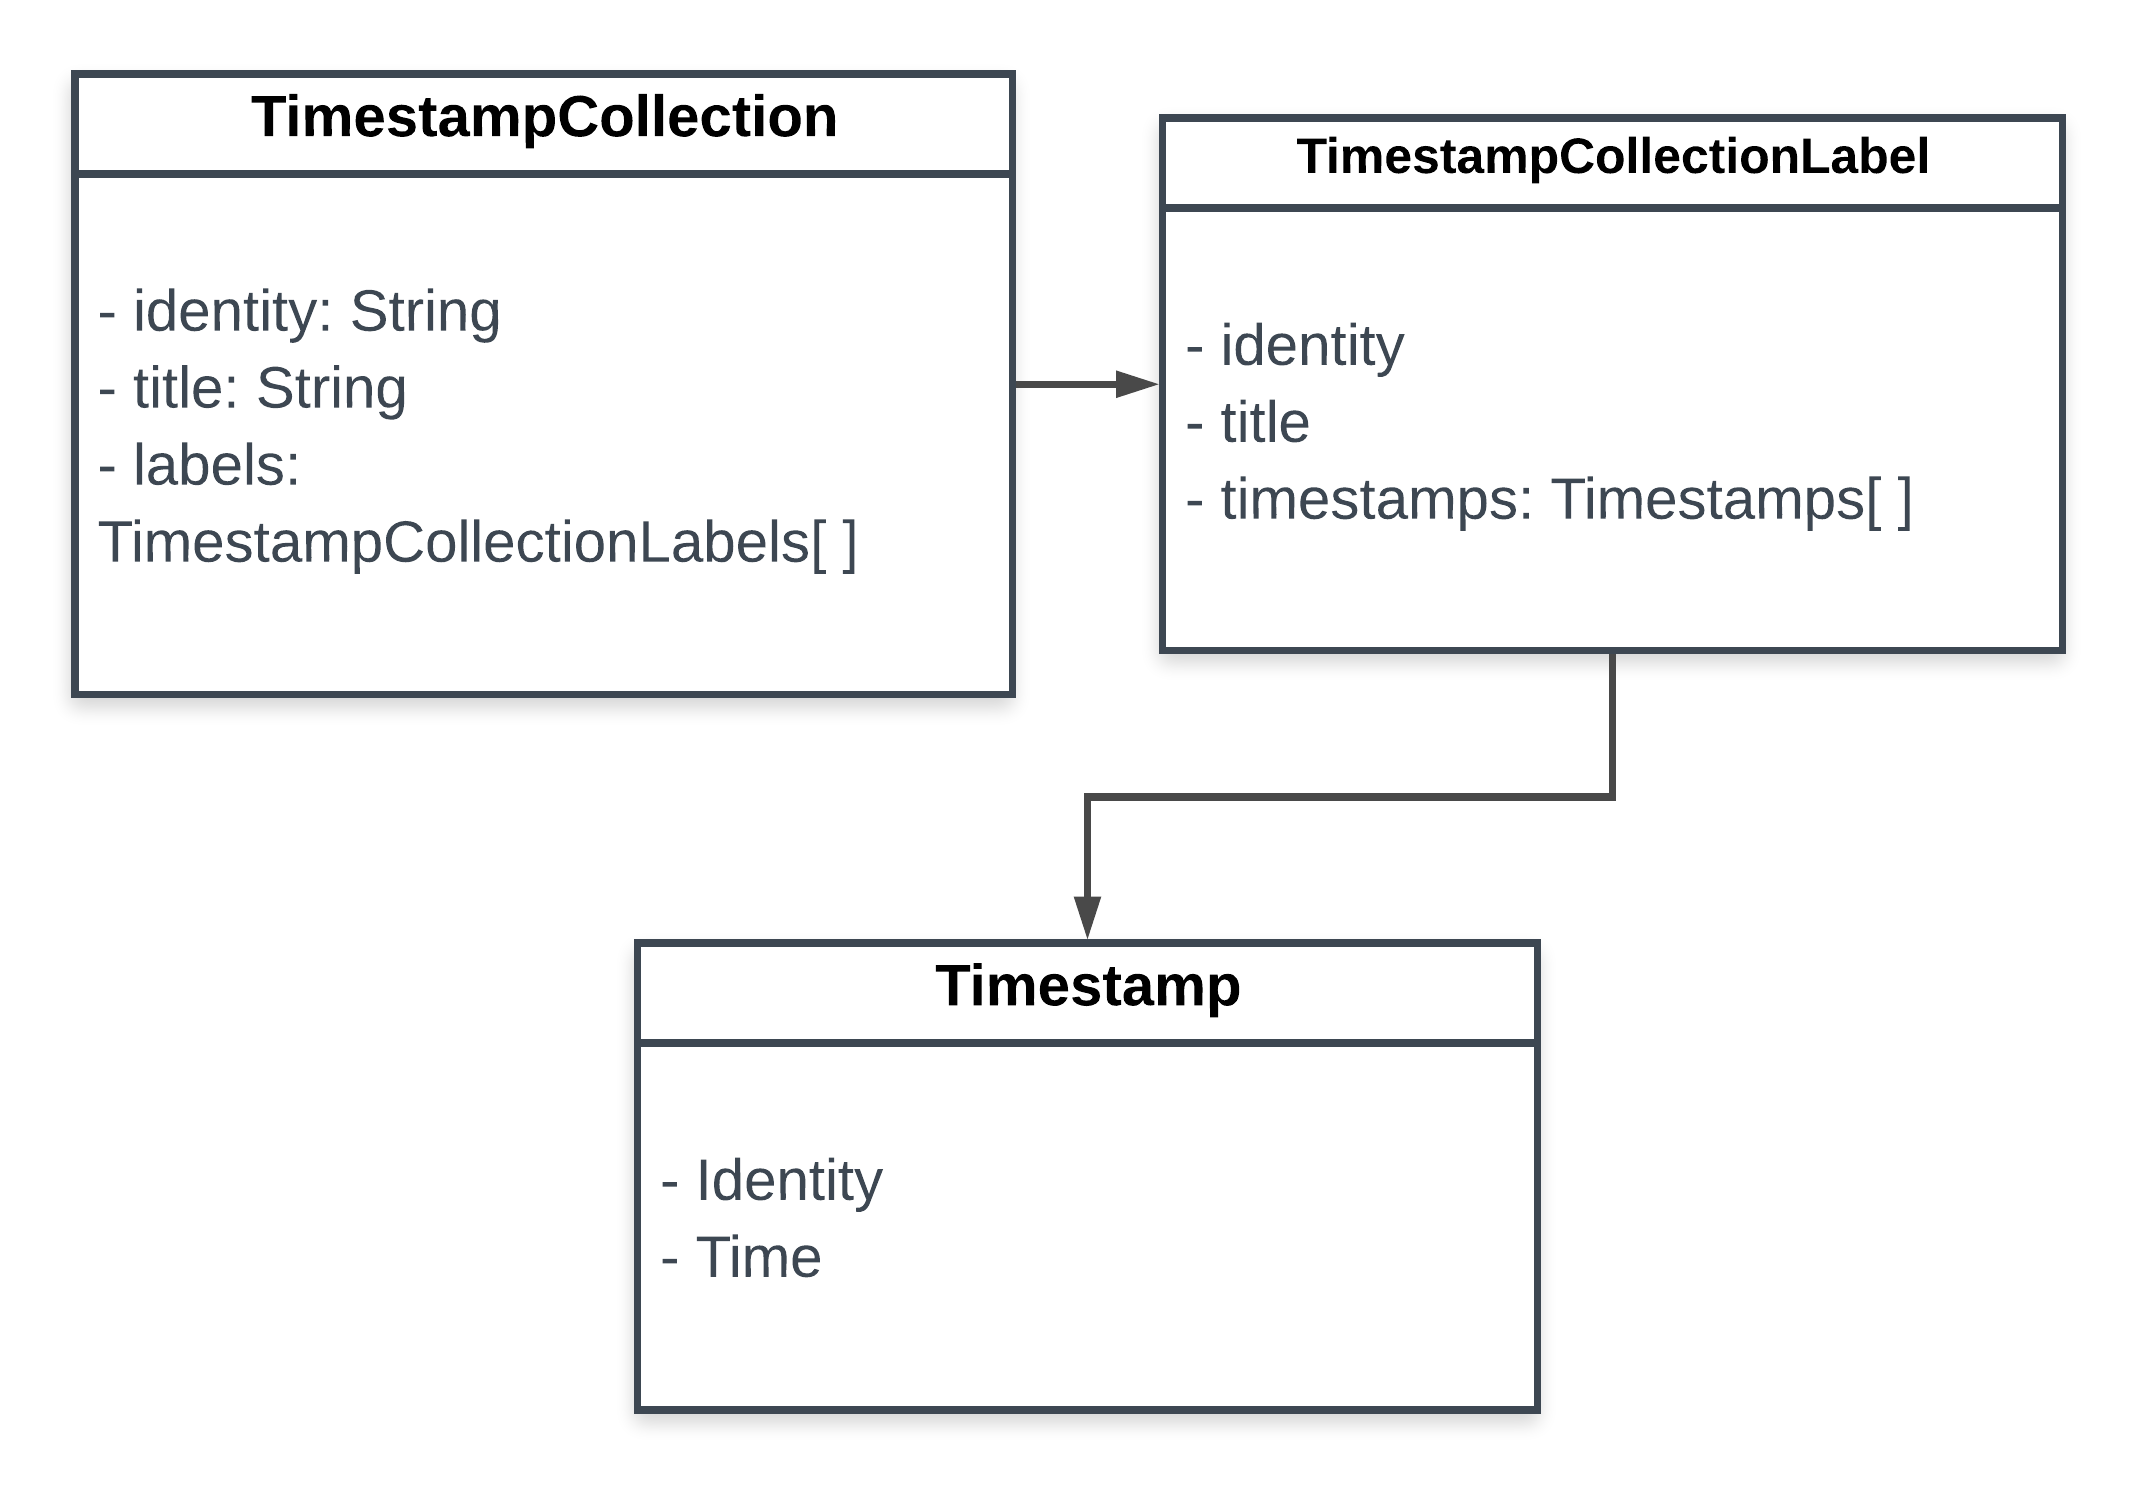
\includegraphics[scale=.15]{img/schema-graph.png}
    \caption{Visual representation of a sample GraphQL Schema}
    \label{fig:schema-graph}
\end{figure}

Figure \ref{fig:schema-graph} is a visual representation of a GraphQL schema with three types, TimestampCollection, TimestampCollectionLabel, and Timestamp.  The edges between each type show that relationships exist between the types. These relationships  would allow the user to create a request as shown in Figure \ref{fig:basic-query}.  The result of this query would be all TimestampCollections with their associated labels and timestamps.  If some of those requests fields or connected data not are needed, however, any part of that query could be removed and the API would respond with less data.

\begin{figure}
    \begin{verbatim}
query {
    timestampCollections {
        identity
        title
        labels {
            title
            timestamps {
                time
            }
        }
    }
}
    \end{verbatim}
    \caption{A basic GraphQL query}
    \label{fig:basic-query}
\end{figure}

\subsubsection{GraphQL vs. SQL}

SQL is debatably one of the most popular querying languages thanks to the popularity of relational databases, which will be discussed more below.  While the aim of this project is to connect GraphQL and SQL queries, it should be noted that the two languages exist for very different reasons.

SQL is a language very strongly tied to the storage and retrieval of data.  Queries act on specific tables that have strictly defined and structured data.  The SQL language does not make sense outside of the context of a relational database.  GraphQL on the other hand is completely agnostic to how the data is stored/retrieved.  The data source could be a relational database, a non-relational database, some other API, or could be programmatically generated. To fetch and update all of this data, GraphQL servers implement functions called resolvers that "resolve" the requested information from a data source.  That data source may be a  database, some other function in the code base, or calling another remote service..  Because of this flexibility, it is possible to use GraphQL as the query language for the front end of the application, such as the web browser or the user software, and SQL as the query language used by a GraphQL server to fetch or update data in a database.
\subsection{REST API}
In 2000, Roy Fielding wrote a PhD thesis focusing on the software architecture of web applications \cite{fieldingArchitecturalStylesDesign2000}.  In this dissertation, Fielding defined a style of designing web servers called Representational State Transfer (REST).  Since then, REST APIs have been the de facto standard for organizing services that send data over the internet.  Whether it is requesting individual web pages or bits of data to be used in an application, REST design patterns are often used. 

To this day, the basic constraints laid out in Fielding's dissertation are still used as the tenants of well designed RESTful interfaces.  A quick google search of REST principles will bring up hundreds of blog posts and tutorials summarizing these guidelines. For more information about REST, the reader is encouraged to do this additional research, however, I will include a brief summary below of the basic rest principles.

\subsubsection{REST Principles}

\begin{itemize}
    \item \textbf{Client-Server:} There should be a division between the software that stores and retrieves data and the software that displays the data.
    \item \textbf{Stateless:} All of the data required to respond to the request should be contained in the request. The server should not store the state of its interaction with the client. That is the client's responsibility.
    \item \textbf{Cache:} The results of a server request should be labeled as cacheable or non-cacheable.  Cacheable requests should not be re-requested for a certain time period to improve network efficiency.
    \item \textbf{Uniform Interface:} All REST services should respond in a uniform way, with each resource having a Unique Resource Identifier (URI).  Through these standard interfaces, web browser can go to nearly any web page without specific configuration.
    \item \textbf{Layered System:} The client is only aware of the top most layer of a REST system, but there may be many layers beneath the public facing layer that process the request.
    \item \textbf{Code-On-Demand:} The client can request code that extends the functionality of the application.  This is the basis of how browsers work.  They request code in the form of HTML, CSS, and JavaScript, which run on the machine and also often continue to request more code.
\end{itemize}

Thankfully, most of these principles are handled without much interference by the modern day developer. Caching, Layered Systems, and Code-On-Demand, are all key aspects implemented by web browsers and operating systems.  What takes most of the work on the developer's part is the organization of data into a Uniform Interface. In a REST API, if I want to request the TimestampCollection with an id of 1, the URI I use to request that resource might be \Verb"/api/timestampCollections/1".  Often, I would retrieve that information using an HTTP GET request.  An edit to that resource might then come through a PUT or DELETE request.

\subsubsection{REST vs. GraphQL}
For how often GraphQL is talked about as an alternative to REST APIs, it should be noted that many of REST's principles are typically implemented in a GraphQL API.  GraphQL servers respond to requests from client programs, GraphQL requests are often cached by their clients, such as the Apollo GraphQL client, and the web servers that respond to GraphQL requests are stateless and behind layered systems.  The biggest deviations from REST are in the fact that the organization of a GraphQL API is not through a Uniform Interface. In GraphQL all allowed queries and mutations are sent through a single `/graphql` endpoint.  Those requests then have a query name or mutation name attached to them that the GraphQL server interprets and knows how to respond to the client.  This allows for a much more flexible, but necessarily uniform, interface; however, since all requests are still over HTTP, a simple JavaScript client can allow almost any web page to interact with a GraphQL server.
\subsection{Modern JavaScript}

The original version of JavaScript was created in 1995 for the Netscape 2.0 browser and was prototyped in only ten days by Brendan Eich \cite{redhatinc.CreatingJavaScript}.  An article published in December of that year claimed that the new language designed for beginner programmers would make it easy for developers to interact with HTML and create web applications \cite{bucholtzNewLanguageAims1995}.  The language has since evolved greatly from that initial design.  The syntax has expanded, new environments for running JavaScript, known as run-times, have become standard, and whole variants of the language have been released and skyrocketed in popularity.  In this section, I aim to cover a few of the general developments in JavaScript as well as describe specific technologies that are utilized in my project.

\subsubsection{Node.js}
When designing applications that run on servers and machines, instead of in browsers, JavaScript, for many years, would have been seen as an unconventional choice.  Fourteen years after JavaScript's initial release, the release of Node.js changed this paradigm as it allowed running JavaScript outside of browsers. When the Google Chrome Project released its significantly improved V8 run-time for JavaScript, the engine was adapted into a server-side execution environment for JavaScript \cite{pramodEpisodeInterviewRyan}.  In an interview on the podcast "Mapping the Journey," Ryan Dahl, the creator of Node.js, claimed that he saw the asynchronous aspects of JavaScript, and the fact that it ran on a single thread, as making the language a perfect candidate for a robust, scalable, server-side language.  By simply adapting the browser's JavaScript engine to run locally on a machine, he unleashed JavaScript to the server environment.

Since then, Node.js and JavaScript have continued to grow in popularity. In last year's Stack Overflow developer survey, JavaScript was the most commonly used programming language and Node.js was the largest non-web/non-browser framework \cite{stackoverflowStackOverflowDeveloper}.

When discussing Node.js, the most important thing to understand is that it is simply a run-time to execute JavaScript on a machine without using a browser.  In practice, it has enabled JavaScript to become a first-class scripting language with full access to file systems, compiled libraries, and a dedicated developer community.

\subsubsection{TypeScript} \label{sec:typescript}
While Node.js adapted JavaScript for the server environment, a few years later, another technology, TypeScript, was created to adapt JavaScript to solve a different issue: static typing.  In its pure form, JavaScript is not a typed language, meaning that variables have no types, such as integers, strings, etc.  The variables are instead dynamic in type, which allows for great flexibility.  As Microsoft began working on web applications and started talking with their customers, however, they realized that JavaScript's lack of typings made managing large applications difficult.  One can imagine that as a code base grows, if there is no compilation step, small adjustments to the shape or type of data stored in variables or functions could be hard to catch.  With errors only surfacing at run-time, these applications became tough to maintain.  Microsoft's solution to this was to create TypeScript, a statically typed JavaScript variant \cite{idgnewsservicestaffMicrosoftAugmentsJavaScript2012}.

When writing in TypeScript, the syntax is nearly identical to JavaScript except variable declarations and function definitions also include types.  Before running a TypeScript program, this code is run through a compiler to ensure that all code is correctly using these typed objects. What makes TypeScript somewhat irregular amongst typed languages is that these types are completely removed at compilation time. The advantage to this is that TypeScript and JavaScript code are fully compatible.  Any TypeScript developer can thus take advantage of existing JavaScript libraries, and JavaScript developers are not required to adopt TypeScript to use these recently developed libraries.  As the developer writes their code, however, these types still exist, so IDEs and text editors can take advantage of the existing types to perform auto completion and check types inline.

Along with typings, TypeScript has also made other syntactic improvements over pure JavaScript.  The core feature utilized by this project has been the decorator syntax.  Introduced in version 1.5 of the language, TypeScript included this syntax while the feature was still in the proposal stage for future JavaScript support \cite{turnerAnnouncingTypeScript2015}.

In programming languages, reflection is the ability for a program to analyze and modify itself during run-time \cite{malenfantTutorialBehavioralReflection1996}.  In TypeScript, one of the common forms of reflection is using decorators to attach metadata to classes, properties, methods, and parameters.  By using a package called \Verb!'reflect-metadata'!, the program can reflect on itself to process the attached metadata and modify its behavior.  To illustrate this idea, I will introduce the server framework used in this project, Nest.js, which heavily relies on the use of decorators.

\subsection{Nest.js} \label{sec:nest-js}
Nest.js is a framework for creating server-side applications in JavaScript or TypeScript.  Along with Angular, the front-end framework that has heavily influenced Nest.js's design, the framework is object-oriented and uses metadata and decorators to declare the structure of the web server.

For example, imagine a simple web server that just responds to one HTTP GET request with a success message.  To define this endpoint, in Nest.js, the program must simply define a Controller, a class that responds to a number of HTTP requests, and a specific method to handle that request.

\begin{figure}
    \begin{verbatim}
import { Controller, Get } from '@nestjs/common';

@Controller('/api')
export class AppController {

    @Get()
    async respondToGetRequest() {
       return {success: true};
    }
}
    \end{verbatim}
    \caption{A simple Nest.js Controller}
    \label{fig:nest-controller}
\end{figure}

In Figure \ref{fig:nest-controller}, we see two examples of decorators: \Verb!@Controller! and \Verb!@Get!.  The former is what tells Nest.js that this class will have functions that respond to HTTP requests on the route \Verb!'/api'!.  The latter marks the function as the code that will return a response for a GET request on the route \Verb!'/api'!.  When these decorators are executed at run-time, they store metadata flagging the class as a controller and the function as an HTTP request method.  The Nest.js framework then reflects on the established metadata and routes the received HTTP requests to the appropriate functions.

As the framework has developed, numerous other features have been implemented and abstracted using decorators, such as request validation, authorization, and GraphQL definitions and resolving.

\section{Motivation}

\subsection{Practice Liszt}
My discoveries related to GraphQL began with a project I called Practice Liszt.  The main goal of the application was to be a rehearsal tool for musicians. As a percussionist, I found it difficult to practice along with video or audio excerpts on applications such as YouTube or Spotify.  As I would try to practice with sometimes 30 or 45 minute long videos, I would have to write down the times of different sections within a piece.  For example, if I wanted to start my practice at the beginning of as second movement of a piece, I would have to write down the time that occurs in the video, scrub to that time, and then start the video with enough time to pick up my instrument/implements and begin playing.

My intended vision for the project was to build a web application where one could create timestamps in these lengthy pieces of audio or video and keep them in an easily accessible list, hence the pun ``Practice Liszt.'' In the Spring of 2018, I did some basic research into the feasibility of this project.  I confirmed that the YouTube API had adequate controls to change the time of YouTube videos, that the interface could be easily created in React.js, a JavaScript UI Framework, and that GraphQL would be an appropriate means of communicating between the front-end (browser) of the application and the back-end (server and database) of the application.

After this initial mock-up, however, I did not work on the project again until the spring of 2019.  At the time I was interviewing for an intern position at the Kalamazoo company Maestro.  For my interview process, I had to implement a project that could show off my skills as a web developer.  Knowing I wanted to tackle this project in the future, I used this as an opportunity to create a complete prototype of the application.  By the end of the week, I had a working prototype that used React, GraphQL, and a non-relational database to store the timestamps called MongoDB.

Thankfully, the software team at Maestro was impressed by my project and I was offered an internship to work there. Going into the summer, I had planned on continuing to work on the project, from a feature standpoint, while I was not working at Maestro.  Ultimately, my goal was to have an application that was not only simple for a musician to use, but could also support use in academic research. On the musician side, they could create timestamps in multiple versions of a piece (think two different recordings, or a video and a piece of audio), and could set up privacy features which would allow them to either keep their timestamps private or share them with others.  For academics, I hoped that they would be able to look at what pieces have been timestamped and by extension, what recordings are associated with which pieces and what spots in the pieces are commonly timestamped.

To achieve this academic side of the project, I realized in July that I needed to redesign the data model.  In order to associate timestamps with actual published pieces of music, I decided to integrate my database with the MusicBrainz database, which is an open source database of music metadata, such as published works, composers, dates, and numerous other bits of data.  This database, however, was structured as a PostgreSQL database.  For this reason, my database went under a complete re-write between July and August to handle data retrieval from a relational SQL database instead of a non-relation database.  In the process of manually writing the resolvers which took GraphQL queries and responded with the appropriate data, I became frustrated with the need to manually define SQL queries that resolved a GraphQL query.  As I learned more at my internship with Maestro, I felt compelled to find a solution that would minimize the amount of work involved in mapping a GraphQL query to the data in a relational database.

\subsection{Maestro}
In June 2019, while working on my Practice Liszt project, I started working at Maestro. My main project over the summer was refactoring the back-end code for a learning management system called Loop.  Our goal  for the project was to move all of the existing code for the web server into the Nest.js framework (see Section \ref{sec:nest-js}).  In this process though, we used the refactor as an opportunity to remove a lot of duplicated logic throughout the code base.  Logic around data validation, processing HTTP requests, and permissions/authorization were all redesigned within the project to be more standard and less repetitive.

At the end of the processes, however, a lot of logic was still duplicated throughout the entire application.  Since the application has been written to have static REST endpoints, for every endpoint, we have to define exactly what data should be returned and how to fetch that from the database. With over two hundred endpoints, this creates code that is often doing the same thing, just in slightly different ways.  Moreover, whenever the front end of the application needs different data, a back-end developer has to make a change to the code to manually change or reformat the returned data.

As a developer at Maestro, while I was working on this refactoring project, I was also given the opportunity to participate in bi-weekly ``Developer Days.''  Somewhat inspired by Google's 20\% time, every other Friday, developers were encouraged to use their work days to work on any kind of software projects they were interested in.  The goal of the day was not to contribute productively to current projects, but to allow developers to explore topics and technologies that they were interested in.

Through my summer as an intern, I spent a number of my Developer Days focused on this idea of automated GraphQL/SQL queries. While I approached this problem from the perspective of my Practice Liszt project, the applicability to work projects became clearer the longer I worked on refactoring the Loop web server.  As I continued to share my progress from Developer Days, my coworker's interest in the project continued to grow and discussions began to occur about how we could potentially integrate this into future projects.  At the time of writing, our hope is that this system could be our standard way of exposing data from a relational database.

\section{GraphQL Query Mapping}

\subsection{Schema/Data Model}

The first step to mapping GraphQL queries to SQL queries is to define a shared schema between the allowed objects that can be requested in GraphQL and the tables in the relational database.  If the GraphQL schema and the database schema are defined in the same way, then each table in database becomes a GraphQL type that a client can request.

The first major design question was how to define these schemas at the same time.  In the JoinMonster library, the data model is only declared for the GraphQL schema and then the developer defines a map from the GraphQL types to SQL Tables \cite{carlJoinMonster}.  This way, the application can join the two tables together and resolve related data.  On the other hand, in Hasura, the GraphQL schema and the database schema are one in the same.  As you define the table schema that Hasura will use to generate SQL tables, a GraphQL schema is generated alongside it \cite{hasurainc.HasuraGraphQLEngine}.

In my solution, similar to Hasura, the data model for the GraphQL schema and the database schema are declared at once, however, they are declared in code instead of in a web interface.  To do this, I am integrating two libraries together: \Verb!type-graphql! for the GraphQL schema and \Verb!sequelize! for the database schema.  Thanks to another package called \Verb!sequelize-typescript!, both of these libraries allow for defining the schema using TypeScript decorators (see Section \ref{sec:typescript}).  As a result, by decorating a single, class that defines the schema for the data, I am given a GraphQL schema that defines that data is available, and a schema that used to make requests to the database.

\begin{figure}
    \begin{verbatim}
@ObjectType()
@Table({
    tableName: 'timestamp_labels',
    underscored: true
})
export class TimestampLabel extends CreatedByEntity<TimestampLabel> {

    @ForeignKey(() => TimestampCollection)
    @Column({
        type: Sequelize.BIGINT,
        field: 'timestamp_collection_id'
    })
    timestampCollectionId: number;

    @Field()
    @Column({
        type: Sequelize.STRING,
        field: 'title',
        allowNull: true
    })
    title: string;

    @Field()
    @Column({
        type: Sequelize.INTEGER,
        field: 'position'
    })
    position: number;

    @Field(() => TimestampCollection)
    @BelongsTo(() => TimestampCollection)
    timestampCollection: TimestampCollection;
}
    \end{verbatim}
    \caption{An example GraphQL/Database Schema}
    \label{fig:example-entity}
\end{figure}

Figure \ref{fig:example-entity} is based on an example from a \Verb!type-graphql! example project and shows how simple it is to define the schema.  The decorator \Verb!@ObjectType()! establishes the class as a GraphQL object type and the \Verb!@Table()! decorator says which table this object type maps to in the database.  Within the class, each \Verb!@Field()! decorator marks the property as being accessible in the GraphQL schema and each \Verb!@Column()! maps the field to a specific column in the database.  The \Verb!@BelongsTo()! decorator is what defines the relationship between two ObjectTypes/Tables.  This metadata is what is eventually used to join the tables together.

\newpage
\setcounter{page}{1}
\printbibliography
%\addcontentsline{toc}{section}{References}
%\bibliographystyle{plain}
%\bibliography{references}
\end{document}
